%%%\documentclass[%
%%%%reprint,
%%%%superscriptaddress,
%%%%groupedaddress,
%%%%unsortedaddress,
%%%%runinaddress,
%%%%frontmatterverbose, 
%%%preprint,
%%%%showpacs,preprintnumbers,
%%%%nofootinbib,
%%%%nobibnotes,
%%%%bibnotes,
%%% amsmath,amssymb,
%%%%aps,
%%%%pra,
%%% prb,
%%%%rmp,
%%%%prstab,
%%%%prstper,
%%%floatfix,
%%%%nolongbibliography
%%%]{revtex4-1}

\documentclass[review,authoryear,12pt]{elsarticle_summary_report}
\usepackage[top=1.0in, bottom=1.0in, left=1in, right=1in]{geometry}


%%%%%%%%%%%%%%%%%%%%
%\usepackage{amsfonts}
%\usepackage{amssymb}
%\usepackage{MnSymbol}
\usepackage{graphicx}
\usepackage{courier}
\usepackage{psfrag}
\usepackage{amsmath}
\usepackage[usenames]{color}
\usepackage{leftidx}
\usepackage[small]{subfigure}
\usepackage{stmaryrd}
\usepackage{amsthm}
\usepackage{multirow}
\usepackage[table]{xcolor}
\usepackage{natbib}
\usepackage{nomencl}
\usepackage{setspace}
\usepackage{dcolumn}% Align table columns on decimal point
\usepackage{bm}% bold math
\usepackage{pdflscape}
% \usepackage{showkeys}
%%%%%%%%%%%%%%%%%%%%

\usepackage{hyperref}
\hypersetup{
    colorlinks=true,
    linkcolor=blue,
    filecolor=magenta,      
    urlcolor=cyan,
}

% \usepackage[active,tightpage]{preview}
% \PreviewSnarfEnvironment[{[]}]{figure}

\makenomenclature

\graphicspath{ {./Figures/cav_17_results/}
               {./Figures/pillbox_coarse_uniform_results/}   
               {./Figures/geom_inquires_impl/}   
             }

%\renewenvironment{equation}[0]{equation}{equation}

%%%%%%%%%%%%%%%%%%%% Additional Commands
%%%%%%%%%%%%%%%%%%%%
%\numberwithin{equation}{section}  	%%Equation Numbering
%%%%%%%%%%%%%%%%%%%%
\begin{document}

\title{PROGRESS REPORT}% Force line breaks with \\
%\thanks{}%

\author[]{Morteza H. Siboni \\
Gerrett Diamond \\
Cameron W. Smith}
%\ead{email address}

%\author[inst1]{Corresponding Author \corref{cor1}}
%\cortext[cor1]{Corresponding author}
%\ead{ca@email.host.edu}
%\address[inst1]{Department of Mechanical Engineering and Applied Mechanics, University of Pennsylvania, \\ Philadelphia, PA 19104-6315, USA}


\date{\today}



\begin{abstract}
  In this document we provide and update on the current status of the Omega3P project. In particular, the following issues will be addresses. (a) In Memory Integration and Load Balancing, (b) the fully parallel adaptive loop, and (c) the implementation details for replacing the geometry calls in Omega3P  with the corresponding PUMI calls.
\end{abstract}

% \begin{keyword}
% \end{keyword}

\maketitle


% \begin{spacing}{0.5}
% \printnomenclature
% \end{spacing}


\section{Introduction}
TODO: Explain The State of Things Before And Summarize The New Things That Have Been Done

\section{Fully Parallel In-Memory \dots}
TODO: Ask Cameron/Gerrett To Fill This Out

\section{Adaptive Loop}
At this stage, we have the adaptation loop in place which consists of the following steps:

\setstretch{0.75}
\begin{itemize}
  \item[] \texttt{while not converged \{ }
   \begin{itemize}
     \item \texttt{partition the mesh with a focus of owned and ghost elements}
     \item \texttt{convert PUMI-mesh to SLAC-mesh}
     \item \texttt{do an Omega3P solve} %could use better wording
     \item \texttt{transfer electric field values to the PUMI-mesh}
     \item \texttt{check for convergence}
     \item \texttt{run Super-convergent Patch Recovery (SPR) -> error estimation -> size field}
     \item \texttt{convert 2nd order Lagrange to 2nd order Bezier}
     \item \texttt{run the curve adapt}
     \item \texttt{convert 2nd order Bezier back to 2nd order Lagrange}
   \end{itemize}

 \item[] \texttt{  \} }
\end{itemize}
\setstretch{1.5}
It is important to emphasize that, the current adaptive loop improves upon the previously available adaptive loop (implemented by Kai) in that it is fully parallel, which required repartitioning a serial mesh after parallel adaptation.


Figures \ref{pill} and \ref{cav} show two working examples for the curve adaptation loop.
\begin{landscape}
\begin{figure}[ph!]
\centering
\subfigure[]{\label{pill_init}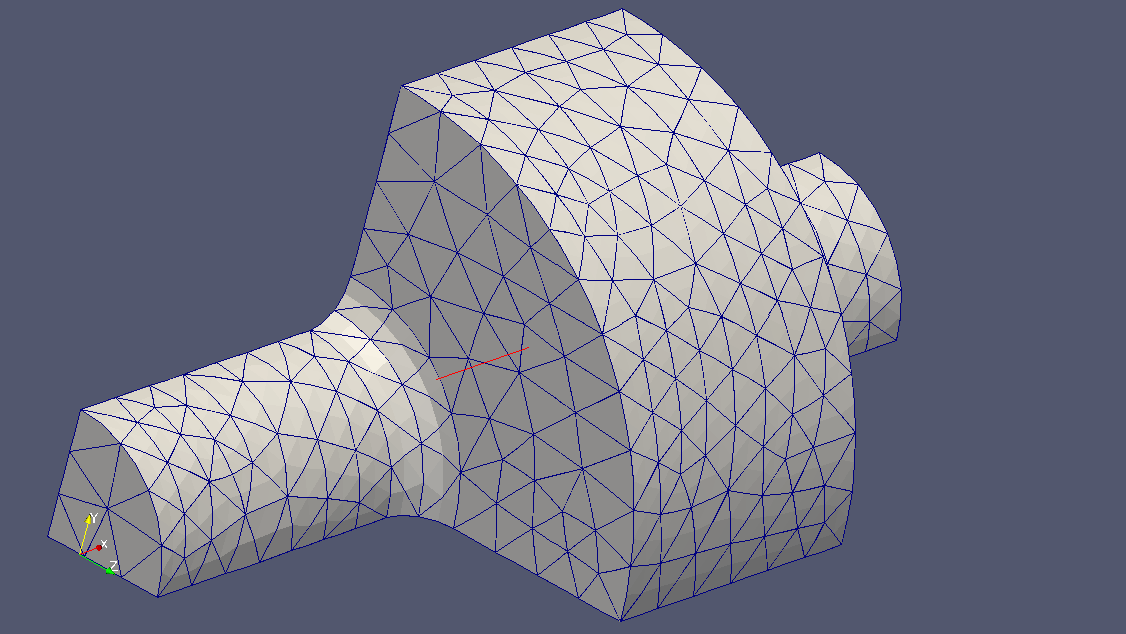
\includegraphics[width=0.55\textwidth]{al_0_ar_0p0125_3721_elems.png}}
\hspace*{50pt}
\subfigure[]{\label{pill_size}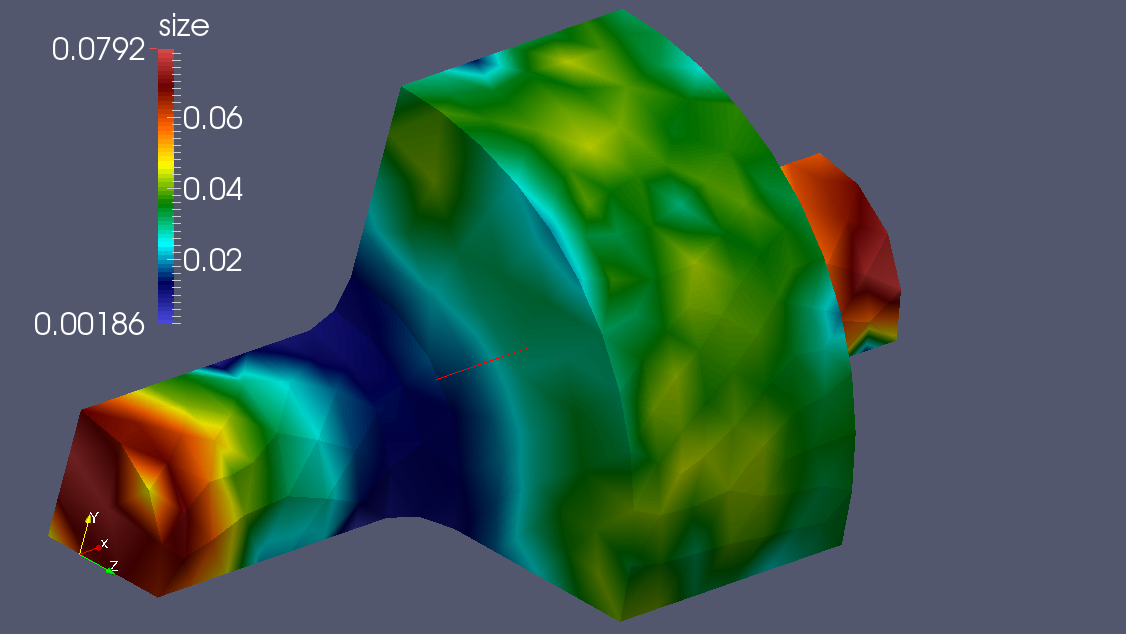
\includegraphics[width=0.55\textwidth]{al_0_ar_0p0125_3721_elems_size_field.png}}
\\
\subfigure[]{\label{pill_adapt}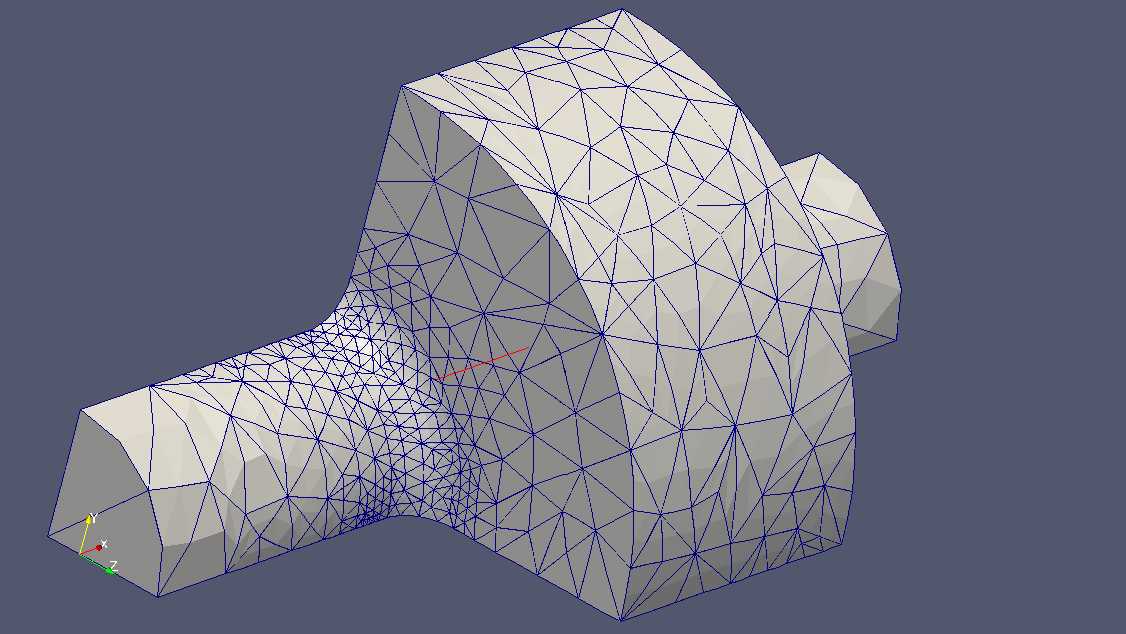
\includegraphics[width=0.55\textwidth]{al_3_ar_0p0125_14221_elems.png}}
\hspace*{50pt}
\subfigure[]{\label{pill_field}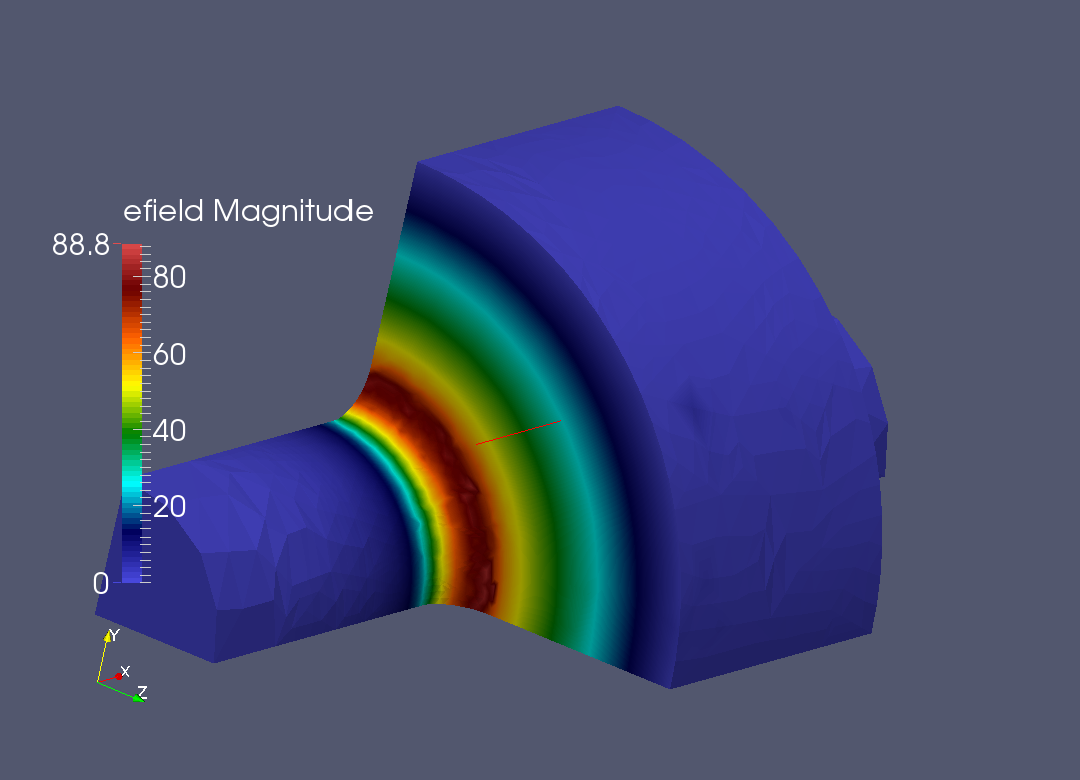
\includegraphics[width=0.55\textwidth]{al_3_ar_0p0125_14221_elems_e_field.png}}
\caption{\label{pill} This Figure shows the results for the PILLBOX model. (a) shows the initial mesh [$\sim3.7\text{K}$ elements], (b) shows the initial size-field, (c) shows the adapted mesh after 3 adaptation steps [$\sim14\text{K}$ elements], and (d) shows the electric field for the final adapted mesh.}
\end{figure}
\end{landscape}
\begin{landscape}
\begin{figure}[ph!]
\centering
\subfigure[]{\label{cav_init}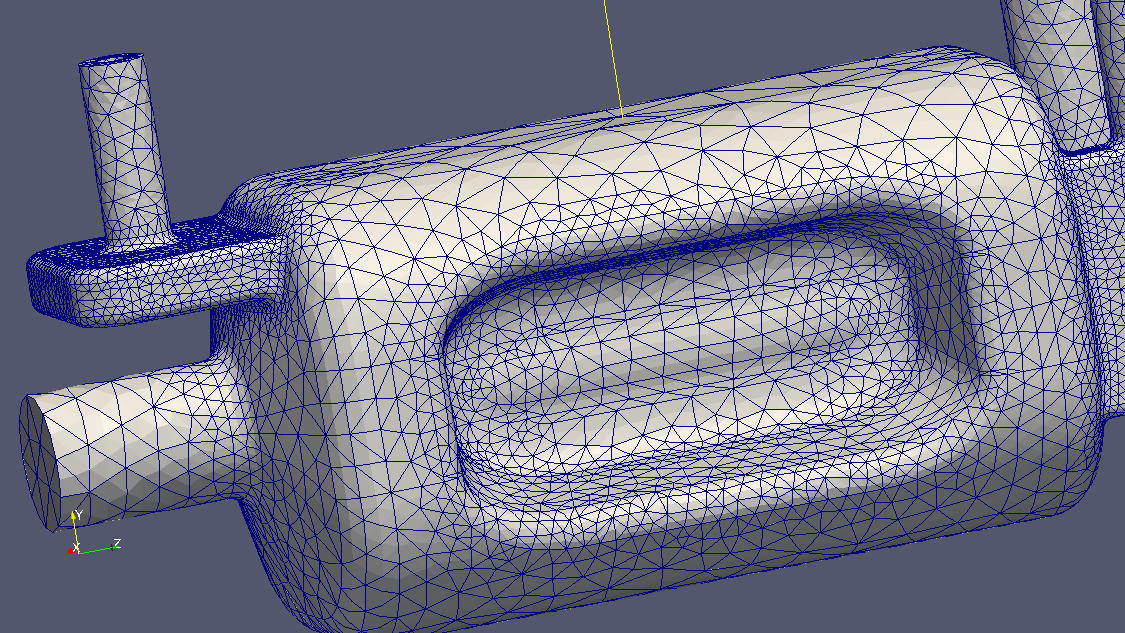
\includegraphics[width=0.55\textwidth]{al_0_ar_0p0125_126044_elems.png}}
\hspace*{50pt}
\subfigure[]{\label{cav_size}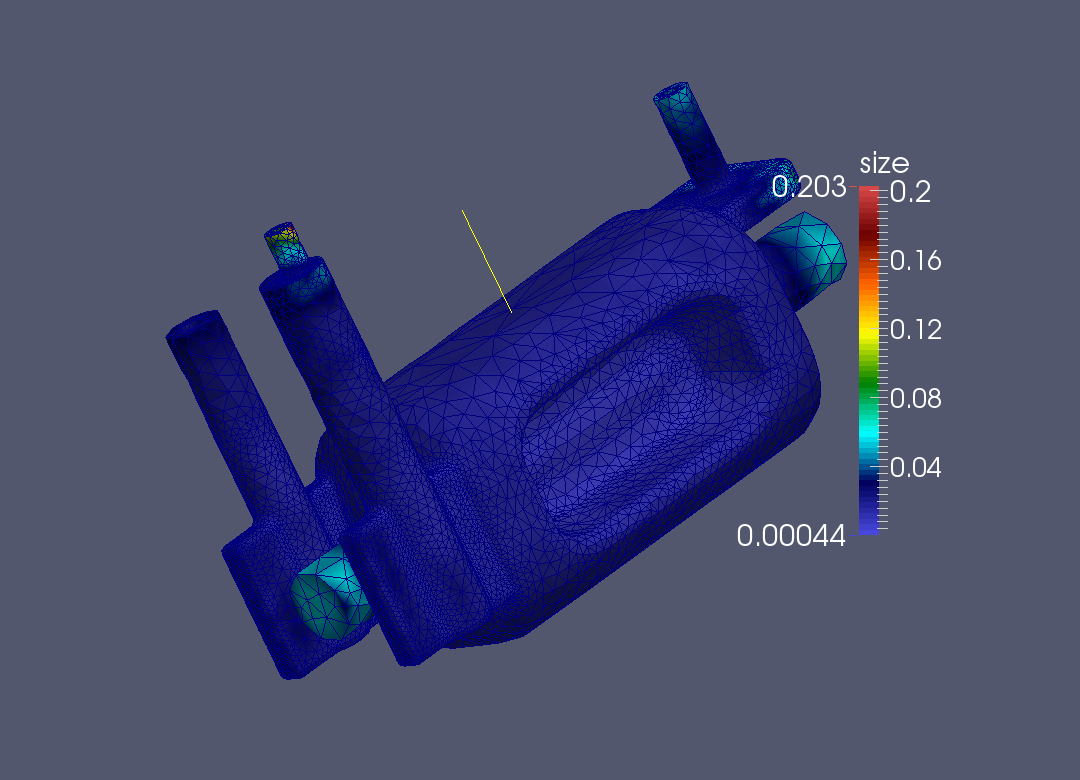
\includegraphics[width=0.55\textwidth]{al_0_ar_0p0125_126044_elems_size_field.png}}
\\
\subfigure[]{\label{cav_adapt}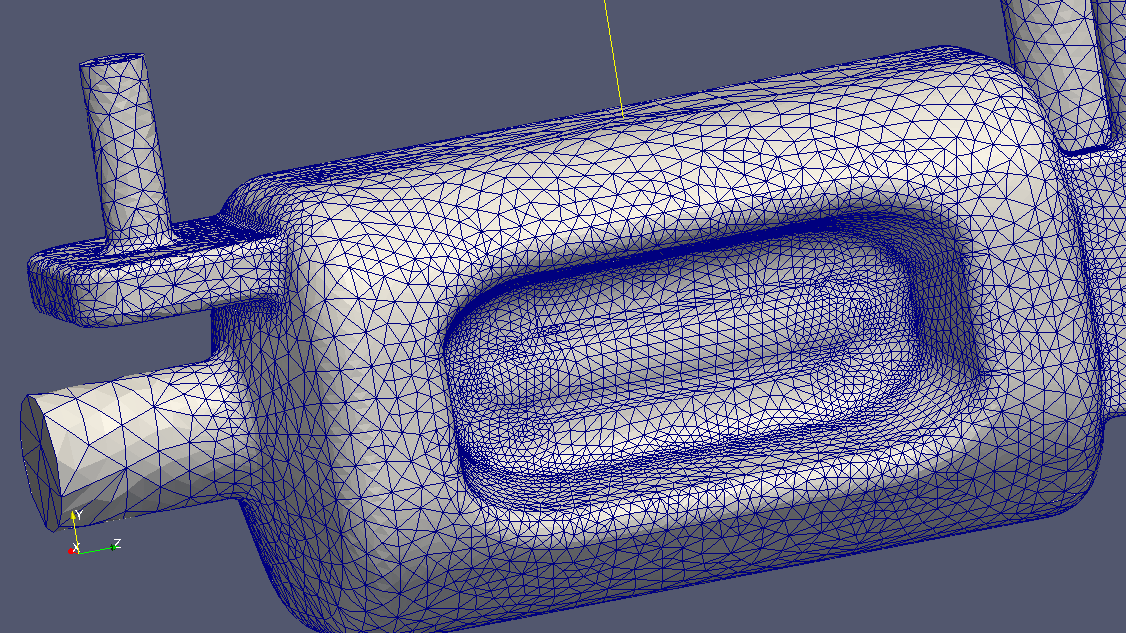
\includegraphics[width=0.55\textwidth]{al_3_ar_0p0125_386896_elems.png}}
\hspace*{50pt}
\subfigure[]{\label{cav_field}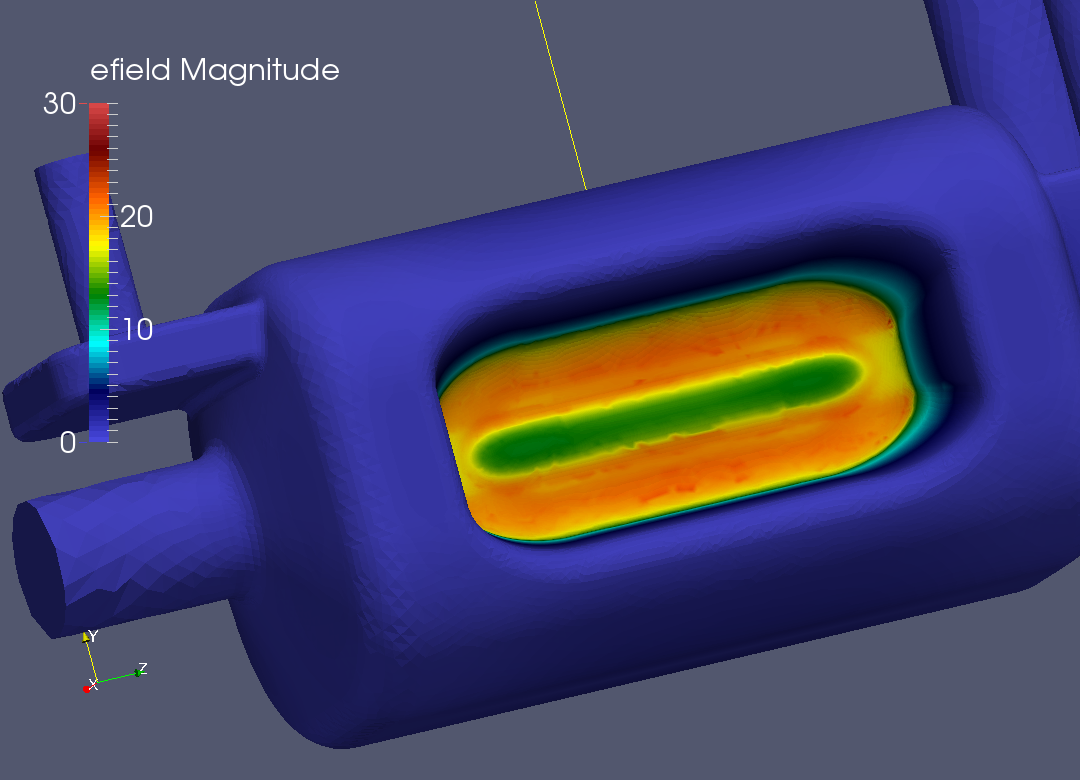
\includegraphics[width=0.55\textwidth]{al_3_ar_0p0125_386896_elems_e_field.png}}
\caption{\label{cav} This Figure shows the results for the CAV17 model. (a) shows the initial mesh [$\sim126\text{K}$ elements], (b) shows the initial size-field, (c) shows the adapted mesh after 3 adaptation steps [$\sim380\text{K}$ elements], and (d) shows the electric field for the final adapted mesh.}
\end{figure}
\end{landscape}
In particular, Fig. \ref{pill} shows the results for the smaller ``PILLBOX''. We start with a uniform and relatively coarse mesh as shown in Fig. \ref{pill_init}. The desired size field for this initial mesh is obtained based on the magnitude of the electric filed and it is shown in Fig. \ref{pill_size}. The final, adapted mesh (for this specific example we needed 3 levels of adaptation) is shown in Fig. \ref{pill_adapt}. Figure \ref{cav} shows the corresponding result for the larger ``CAV17'' model.


\section{Moving Towards Higher-Order Geometries}
As a first step towards using higher-order geometric elements, we have been able to replace the Omega3P calls to compute determinant of the Jacobian with the corresponding PUMI calls. This is done by storing and additional pointer in each Omega3P-element that points to the corresponding  PUMI-element (see Fig. \ref{imp} for the details of the implementation).
\begin{figure}[ph!]
\centering
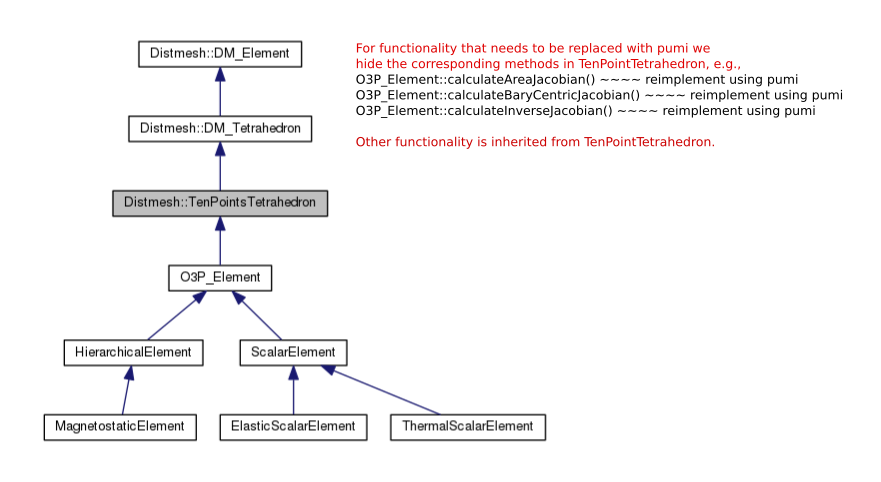
\includegraphics[width=0.95\textwidth]{hide_ten_point_tet.png}
\caption{\label{imp} This Figure shows the implementation details for replacing Omega3P calls for determinant calculation with the corresponding PUMI calls.}
\end{figure}
This, in theory, should make it possible to raise the (geometric) order of the elements. (Currently, we have support for up to 6th order Bezier elements.)

% \section*{References}
% \bibliographystyle{elsarticle-harv_noURL}
% \bibliography{Ref}


\end{document}
